\section{Zielsetzung}
\label{sec:Ziel}

Ziel des Versuches ist es die effektive Masse der Leitungselektronen in einem n-dotiertem Galliumarsenid (n-GaAs) mithilfe des Faraday-Effektes zu bestimmen.
Dazu wird der Winkel $\theta$ zwischen der Polarisationsebene einer einfallenden und der Polarisationsebene einer auslaufenden Richtung gemessen.

\section{Theorie}
\label{sec:Theorie}

\subsection{Die effektive Masse}
\label{subsec:effektiveMasse}

Die effektive Masse beschreibt in der Festkörperphysik die Beschreibung einer Masse eines Teilchens im Rahmen einer semiklassischen Beschreibung. Ähnlich der reduzierten Masse
erlaubt die effektive Masse die Verwendung einer einfacheren Bewegungsgleichung, als mit der realen Masse.
Die effektive Masse folgt aus einer Taylorreihenentwicklung der Elektronenenergie $\epsilon(\vec k)$, mit dem Wellenvektor $\vec k$, 
\begin{align}
    \epsilon(\vec{k})=\epsilon\left(0\right)+\frac{1}{2}\sum_{i=1}^3\left(\frac{\partial\epsilon^2}{\partial k_i^2}\right)_{k=0}k_i^2+...\,.
    \label{eq:Taylor}
\end{align}
In der Taylorreihe \eqref{eq:Taylor} lässt sich der harmonische Oszillator
\begin{align*}
    \epsilon=\frac{\hbar k^2}{2m}
\end{align*}
identifizieren, sofern ein $\hbar$ multipliziert wird. Somit folgt der Ausdruck der effektiven Masse zu
\begin{align}
    m_i^*:=\frac{\hbar^2}{\left(\frac{\partial\epsilon^2}{\partial k_i^2}\right)_{k=0}}\,.
\end{align}

\subsection{Zirkulare Doppelbrechung}
\label{subsec:ZirkulareDoppelbrechung}

Zirkulare Doppelbrechung ist die Fähigkeit eines Kristalles die Polarisationsebene einer liner polarisierten Welle bei Transmission durch ein optisches Medium zu drehen. Grund dafür 
ist, dass die Phasengeschwindigkeiten für links- und rechtszirkular polarisiertes Licht in einem Kristall verschieden sind. Der Winkel zwischen der Polarisationsebene der 
eintreffenden und auslaufenden Welle wird als Drehwinkel $\theta$ definiert. Um ebendiesen Winkel zu berechnen wird die Polarisationsebene einer linear polarisierten Welle, nachdem sie einen 
Kristall der Länge $L$ durchquert hat, in einen linkszirkularen und einen rechtszirkularen Anteil zerlegt, die sich beide in $z$-Richtung ausbreiten.
\begin{align}
    \label{eq:PolAnteil}
    E(z)= \frac 12 \left(E_{\text R}(z)+E_{\text L}(z)\right).
\end{align}
% Mit $k_{\text R}\neq\k_{\text L}$ gilt für die beiden Summanden aus \eqref{eq:PolAnteil},
% \begin{align}
%     E_{\text R}(z)&= (E_0\vec x_0-iE_0\vec y_0)e^{ik_{\text R}z}, \\
%     E_{\text L}(z)&= (E_0\vec x_0+iE_0\vec y_0)e^{ik_{\text L}z}. \\
% \end{align}
Für eine Welle, die bei $z=0$ in den Kristall eintritt folgt, dass die Polarisation parallel zur $x$-Richtung polarisiert ist,
\begin{align}
    E(0)=E_0\vec x_0.
\end{align}
Ein Skizze zur Drehung der Polarisationsebene einer Welle, die von rechts in $z=0$ in den Kristall eintritt und um den Winkel $\theta$ gedreht wird ist in \autoref{fig:DrehungSkizze} 
abgebildet.
\begin{figure}[H]
	\centering
	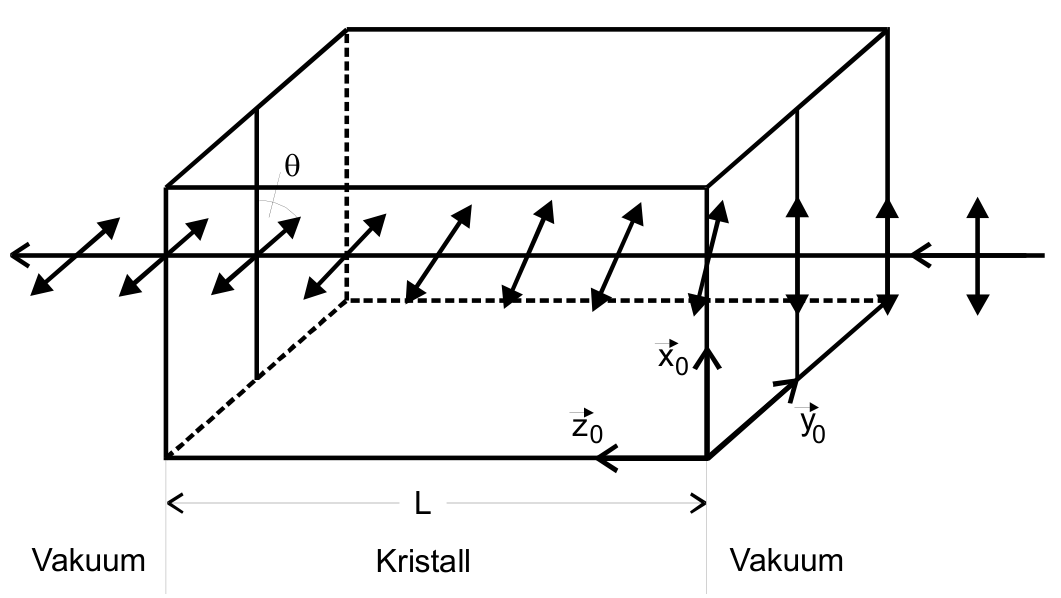
\includegraphics[width=0.6\linewidth]{data/PolarisationDrehung.png}
	\caption{Skizze einer Drehung einer Polarisationsebene.\cite{Anleitung46}}
	\label{fig:DrehungSkizze}
\end{figure}
Mit den Abkürzungen
\begin{align}
    \psi&\equiv\frac 12L(k_{\text R}+k{\text L}), \\
    \theta &=\equiv \frac 12L(k_{\text R}-k_{\text L}),
\end{align}
folgt ein Ausdruck für die Polarisationsebene nachdem eine Welle einen Kristall der Länge $L$ durchquert hat zu
\begin{align}
    \label{eq:PolAusdruck1}
    E(L)=E_0e^{i\psi}(\cos(\theta)\vec x_0+\sin(\theta)\vec y_0).
\end{align}
Ausdruck \eqref{eq:PolAusdruck1} beschreibt eine linear polarisierte Welle an der Stelle $z=L$. deren Polarisation um den Winkel $\theta$ aus der eingehenden Welle gedreht ist.
Die Doppelbrechung der Welle innerhalb eines Kristalles entsteht durch induzierte elektrische Dipolmomente, die sowohl auf die Atome auf den Gitterplätzen, als auch auf die 
Bandelektronen, die in Wechselwirkung mit den Atomrümpfen stehen, zurück. Es kann sich deshalb nur um induzierte Dipole handeln, da permanente Dipole eine zu große Relaxationszeit 
aufweisen, als dass sie mit dem Wechselfeld einer Lichtquelle interagieren können. 
Die makroskopische Polarisation eines Kristalls lässt sich mit
\begin{align}
    \vec P=\varepsilon_0\chi\vec E,
\end{align}
beschreiben, wobei $\vec P$ die Polarisation selber ist, $\varepsilon_0$ die Influenzkonstante und $\chi$ die dielektrische Suszeptibilität beschreibt. Die dielektrische Suszeptibilität
ist in isotropen Kristallen, wie etwa in Gläsern ohne äußerem Magnetfeld, eine skalare Größe, wohingegen sie in anisotropen Kristallen einen Tensor darstellt. Für doppelbrechende
Materialien treten nicht-diagonale Elemente in dem eigentlich symmetrischen Tensor auf, die komplex konjugiert sind,
\begin{align}
    \chi=
  \left( {\begin{array}{ccc}
   \chi_\text{xx} & \text{i}\chi_\text{xy} & 0\\
   \text{i}\chi_\text{yx} & \chi_\text{yy} & 0\\
   0 & 0 &\chi_\text{zz}
  \end{array} } \right)\,.
\end{align}
Wird die Wellengleichung für eine ebene WElle gelöst, wird gezeigt, dass die Wellenzahl für ebensolche Materialien nur die Werte
\begin{align}
    k_\pm =\frac\omega c\sqrt{(1+\chi_{XX})\pm\chi_{xy}}
\end{align}
annehmen kann. Es folgt somit der folgende Ausdruck für den Drehwinkel
\begin{align}
    \theta\approx \frac{L\omega}{2cn}\chi_{xy}.
\end{align}

\subsection{Der Faraday-Effekt}
\label{subsec:Der Faraday-Effekt}

Der Faraday-Effekt ist die Drehung der Polarisationsebene einer einfallenden Welle in einem optischen Medium, wenn dieses in einem zur Ausbreitungsrichtung der Welle parallelen 
Magnetfeld befindet. Aufgrund der Bandlücke zwischen Valenz- und Leitungsband in der Bandstruktur von Halbleitern, werden Halbleiter mit Fremdatomen versehen, wodurch sich die
elektrische Leitfähigkeit steigert. Solche Halbleiter werden dotierte Halbleiter genannt. Es wird zwischen n-dotierten Halbleitern und p-dotierten Halbleitern unterschieden.
N-Halbleiter, fügen in einem $n$-wertigen Atom $n+1$-wertige Fremdatome auf den Gitterplätzen hinzu, wodurch $n$ Valenzelektronen zum Aufbau der
$n$ kovalenten Bindung genutzt werden kann. Es bleibt dabei ein Elektron über, welches über viele Gitteratome delokalisiert ist und deshalb als frei angesehen werden kann. Es genügt
bereits eine geringe Energie um das delokalisierte Hüllenelektron zu lösen und zu einem Leitungselektron zu machen. Aus diesem Grund werden die Fremdatome auch Donatoren genannt.
Die Energieniveaus der Donatoren sind dicht unter der Leitungsbandkante und können nur mit einem der Zustände besetzt werden. Die bei n-Halbleitern zur Leitfähigkeit beitragenden
Elektronen sind die von den Donatoren ins Leitungsband abgebenen Elektronen, die damit die elektrische Leitfähigkeit erhöhen.
Bei p-Halbleitern werden in ein System aus $n$-wertigen Atomen $n-1$-wertige Fremdatome gebracht, wobei eine der $n$ kovalenten Bindungen nur noch mit einem, anstatt ursprünglich mit
zwei Elektronen, besetzt werden kann. Es entsteht demnach ein Loch, in dem ein Elektron eingefangen werden kann. Die Fremdatome eines p-Halbleiters werden demnach Akzeptoren genannt.
Das Energieniveau der Akzeptoren befindet sich knapp über dem Valenzband und somit tragen überwiegend die Löcher im Valenzband, die durch die Akzeptoren entstanden sind, zur elektrischen
Leitfähigkeit bei.
Die Anwesenheit eines Magnetfeldes erniedrigt die Symmetrie eines Kristalles und so lässt sich zeigen, dass der Drehwinkel der auftretenden Doppelbrechung proportional zur
magnetischen Flussdichte $B$, zur Probenlänge $L$ und zur Zahl de rLadungsträger $N$ pro Volumeneinheit ist,
\begin{align}
    \theta&=\frac{e_0^3\omega^2NBL}{e\varepsilon_0c(-m\omega^2+K)^2-(e_0\omega B)^2n}, \\
    \iff \theta &=\frac{\text{e}_0^3\omega^2NBL}{2\epsilon_0cm^2\left(\left(-\omega^2+K/m\right)^2-\left(\frac{\text{e}_0}{m}B\omega\right)^2\right)n}.
    \label{eq:DrehwinkelDoppelbrechung}
\end{align}
In \eqref{eq:DrehwinkelDoppelbrechung} ist der Faktor $\sqrt{K/m}$ als Resonanzfrequenz $\omega_0$, die bei Halbleitern im Infrarotbereich liegen,  und $\frac{Be_0}{m}$ als 
Zyklotronfrequenz $\omega_c$ zu identifizieren. Unter der Annahme, dass die Messfrequenz weit unterhalb der Resonanzfrequenz liegt, folgt der Fall der quasifreien Ladungsträger, der
im Grenzfall $\omega_0\rightarrow0$ mit $\omega_0>\omega_c$ betrachtet wird, gilt
\begin{align}
    \label{eq:WinkelFrequenz}
    \theta(\lambda)=\frac{2\pi^2\text{e}_0^3c}{\epsilon_0}\frac{1}{m^2}\frac{1}{\lambda^2\omega_0^4}\frac{NBL}{n}.
\end{align}
Wird die Masse des Elektrons $m$ durch die effektive Masse $m^*$ ersetzt und die Faraday-Rotation pro Einheitslange $\theta_{\text{frei}}=\theta/L$ eingefügt, vereinfacht sich
\eqref{eq:WinkelFrequenz} zu dem folgenden Ausdruck,
\begin{align}
    \theta_{frei}=\frac{e_0^3}{8\pi^2\varepsilon_0c^3(m^*)^2}\lambda^2\frac{NB}{n}.
\end{align}